\documentclass[10pt,twocolumn,letterpaper]{article}

% \usepackage{cvpr}              % To produce the CAMERA-READY version
\usepackage[pagenumbers]{cvpr} % To force page numbers, e.g. for an arXiv version

% Include other packages here, before hyperref.
\usepackage{
  pgfplots,
  pgfplotstable,
  tikz
}
\newcommand\xyz{} % in order to use a different macro
\newcommand{\addlegendentrySI}[3][]{%
  \begingroup\edef\x{\endgroup
    \noexpand\addlegendentry{{#2} {#3}}}\x
}
\usepackage{graphicx}
\usepackage{comment}
\usepackage{amsmath}
\usepackage{amssymb}
\usepackage{booktabs}
\usepackage[toc,acronym]{glossaries}
\newacronym{DL}{DL}{Deep Learning}
\newacronym{AI}{AI}{Artificial Intelligence}
\newacronym{RL}{RL}{Reinforcement Learning}
\newacronym{SSL}{SSL}{Self-Supervised Learning}
\newacronym{XAI}{XAI}{Explainable AI}
\newacronym{DRL}{DRL}{Deep Reinforcement Learning}
\newacronym{TD}{TD}{Temporal Difference}
\newacronym{DQN}{DQN}{Deep Q Network}


\usepackage[pagebackref,breaklinks,colorlinks]{hyperref}
\usepackage[capitalize]{cleveref}
\crefname{section}{Sec.}{Secs.}
\Crefname{section}{Section}{Sections}
\Crefname{table}{Table}{Tables}
\crefname{table}{Tab.}{Tabs.}

\newcommand{\umapSubPlotUnColored}[4]{
  \begin{tikzpicture}
  \begin{axis}[
      height=5.5cm,
      ticks=none
    ]
    \pgfplotsforeachungrouped \foridx/\forcol in {1/red,2/violet,3/black,4/purple,5/orange,6/green,7/teal,8/blue} {
      \ifnum\foridx<#3
      \expandafter\addplot\expandafter[only marks,mark options={scale=.5}, fill opacity=.5, draw opacity=0.5] table [col sep=comma] {#2/slide\foridx.csv};
      \fi
      }
  \end{axis}
\end{tikzpicture}
\caption{Model #4}
}

\newcommand{\umapSubPlot}[4]{
  \begin{tikzpicture}
  \begin{axis}[
      height=5.5cm,
      ticks=none
    ]
    \pgfplotsforeachungrouped \foridx/\forcol in {1/red,2/violet,3/black,4/purple,5/orange,6/green,7/teal,8/blue} {
      \ifnum\foridx<#3
      \expandafter\addplot\expandafter[\forcol,only marks,mark options={scale=.5}, fill opacity=.5, draw opacity=0.5] table [col sep=comma] {#2/slide\foridx.csv};
      \fi
      }
  \end{axis}
\end{tikzpicture}
\caption{Model #4}
}



\def\cvprPaperID{*****}
\def\confName{NLDL}
\def\confYear{2023}

% TODO Cite presentations?

\begin{document}
\title{NLDL Winter School 2023}

\author{Candidate 25}
\maketitle
% Computational pathology is study of disease using methods such as artificial intelligence. For building models, there are three main hindrances: 1) lack of publicly available data, 2) large image-size and high number of details d 3) lack of ground truth data due to expert disagreeance. Consequently, developers have to compromise when building a model. To know if models are accurate enough, explainable AI can help. But, are the explanations good enough that a pathologist can trust a model used to evaluate patient diagnosis and/or prognosis? 


\begin{figure*}
  \centering
  \begin{subfigure}[b]{.25\textwidth}
    \centering
    \umapSubPlotUnColored{fig:umapDefaultGood}{uncondition}{3}{$\alpha$}
  \end{subfigure}
  \hfill
  \begin{subfigure}[b]{.25\textwidth}
    \centering
    \umapSubPlot{fig:umap2augDefaultGood}{normalModel}{3}{$\gamma$}
  \end{subfigure}
  \\
  \vspace{1.0cm}
  \begin{subfigure}{.25\textwidth}
    \centering
    \umapSubPlot{fig:conditionFalse}{uncondition}{3}{$\delta$}
  \end{subfigure}
  \hfill
  \begin{subfigure}{.25\tejxtwidth}
    \centering
  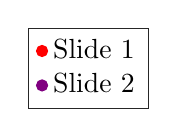
\begin{tikzpicture}
    \begin{axis}[
        hide axis,
        legend style={draw=white!15!black,legend cell align=left},
        xmin=10,
        xmax=90,
        ymin=0,
        ymax=30,
        only marks,
        legend style = {at={(0.20,0.40)}, anchor=west},
        legend entries = {{Slide 1}, {Slide 2}},
        ticks=none]
      \addlegendimage{red};
      \addlegendimage{violet};
      \addlegendimage{black};
      \addlegendimage{purple};
      \addlegendimage{orange};
      \addlegendimage{green};
      \addlegendimage{teal};
      \addlegendimage{blue};
    \end{axis}
    \end{tikzpicture}
  \end{subfigure}
  \caption{UMAP plots from 8 randomly selected tiles from the validation set used in model training. The samples are the same for all graphs}
  \label{fig:umaps}
\end{figure*}

\end{document}
